La adaptación permite obtener una máxima eficiencia en la transmisión de energía, eliminando reflexiones de onda. Dentro de las posibles formas de adaptación, se optó por la utilización del adaptador de cuarto de onda y stub. La línea opera en un entorno de la mínima frecuencia, $\SI{72}{\mega\hertz} < f < \SI{88}{\mega\hertz}$, por lo que se considera el valor de carga de la expresión \eqref{ec.z_80}.

A su vez se considera un criterio de $|\rho_l|<0,2$, ó de forma equivalente $\rm{ROE} \leq 1,5$

\subsection{Adaptador de cuarto de onda}
El proceso consiste en intercalar el adaptador a una distancia $z_s$ de la carga $Z_L$, de forma tal que la impedancia de entrada $Z_{in}$ del conjunto línea y carga sea real. Para hallar el valor de $z_s$ se utiliza la carta de Smith mediante software. El adaptador queda definido mediante los parámetros $z_a$ (impedancia del adaptador) y $L_a$ (longitud del adaptador). La impedancia característica de la línea es dato, $Z_o = \SI{50}{\ohm}$. Ubicandose en $Z_L$, se desplaza hacia el generador sobre la circuinferencia $|\rho_L|$ hasta obtener impedancia real (eje real). Así se obtiene longitud de arco recorrido da la posición $z_s$ del adaptador. A partir de dicho valor y $Z_{in}$ se obtienen los parámetros de la línea \eqref{ec.z_a_4} y \eqref{ec.L_a_4}.

\begin{equation}
	\centering
	Z_a = \sqrt{Z_o \cdot Z_{in}} = \sqrt{ \SI{50}{\ohm} \cdot \SI{1.38}{\ohm} } = \SI{8.3}{\ohm}
	\label{ec.z_a_4}
\end{equation}	

\begin{equation}
	\centering
	L_a = \frac{\lambda_a}{4} = \frac{ \SI{3.75}{\meter} }{4} = \SI{0.937}{\meter}
	\label{ec.L_a_4}
\end{equation}

%%%% FIGURA PARA CUARTO DE ONDA ESPACIO LIBRE
\begin{figure}[H]
	\centering
	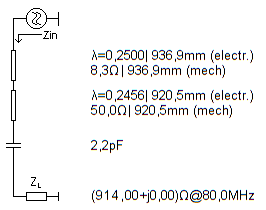
\includegraphics[scale=0.83]{imagenes/smith_4_espacio_libre_esq.png}
	\label{fig.smith_4_esq}
\end{figure}
\begin{figure}[H]
	\centering
	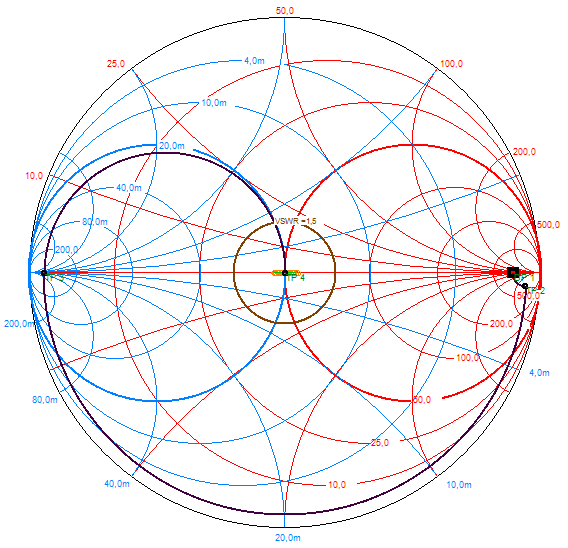
\includegraphics[scale=0.63]{imagenes/smith_4_espacio_libre.png}
	\label{fig.smith_4}
\end{figure}



\subsection{Stub}

La adaptación mediante \texttt{stub} consiste en anexar un trozo de la misma línea conectada en paralelo. Normalmente, para evitar interferencias se suele cortocircuitar el extremo de la carga. Se parte del punto de impedancia obtenido en \emph{4nec2} hasta llegar a la circunferencia de impedancia real unitaria moviéndose hacia el generador. Allí se coloca el stub cuyo largo será el necesario hasta llegar al centro de la carta recorriendo la circunferencia de impedancia real unitaria en sentido antihorario. Utilizando el programa se obtiene:

\begin{equation*}
	\centering
	L_s = \num{0.0269}\cdot \lambda = \SI{100.8}{\milli\m}
\end{equation*}

\begin{equation*}
	\centering
	d_s = \num{0.2195}\cdot \lambda = \SI{822.5}{\milli\m}
\end{equation*}


%%%% FIGURA PARA STUB ESPACIO LIBRE
\begin{figure}[H]
	\centering
	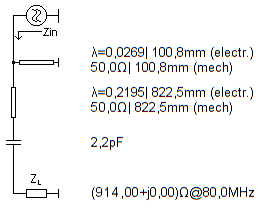
\includegraphics[scale=0.83]{imagenes/smith_stub_espacio_libre_esq.png}
	\label{fig.smith_stub_esq}
\end{figure}

\begin{figure}[H]
	\centering
	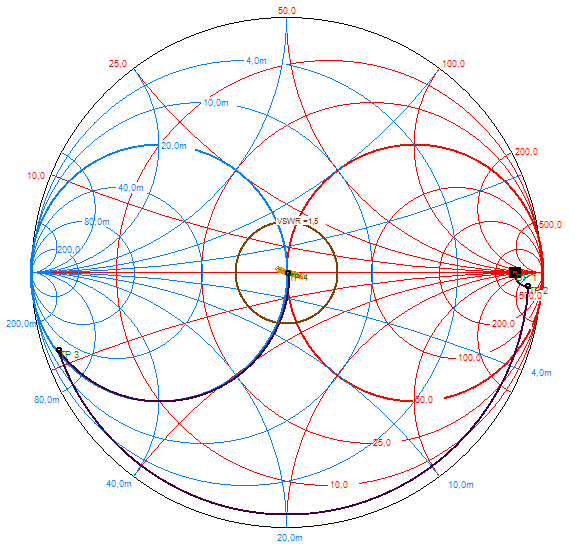
\includegraphics[scale=0.63]{imagenes/smith_stub_espacio_libre.png}
	\label{fig.smith_stub}
\end{figure}



